\subsection{Ütközések feloldása}

%14
\begin{frame}
  Ha több előírás is vonatkozik ugyanannak az objektumnak a formázására, elsőként a forrás prioritása dönt (csökkenő sorrendben):
  \begin{enumerate}
    \item soron belüli formázások
    \item külső és belső (\texttt{<link>}, \texttt{<style>} elemek) formázások
    \item böngésző alapértelmezése
  \end{enumerate}
  Azonos prioritás (pl. két külső stíluslap) esetén a később betöltött szabály felülírja a korábbit.
\end{frame}

%15
\begin{frame}
  \begin{exampleblock}{\textattachfile{utkozes1.html}{utkozes1.html}}
    \scriptsize
    \lstinputlisting[style=HTML,linerange={6-13},numbers=left,firstnumber=6]{utkozes1.html}
  \end{exampleblock}
  \begin{columns}[T]
    \column{0.6\textwidth}
      \begin{exampleblock}{\textattachfile{utkozes1.css}{utkozes1.css}}
        \scriptsize
        \lstinputlisting[style=HTML,numbers=left,firstnumber=1]{utkozes1.css}
      \end{exampleblock}
    \column{0.3\textwidth}
      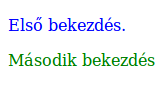
\includegraphics[width=.66\textwidth]{utkozes1.png}
  \end{columns} 
\end{frame}

%16
\begin{frame}
  \begin{exampleblock}{\textattachfile{utkozes2.html}{utkozes2.html}}
    \scriptsize
    \lstinputlisting[style=HTML,linerange={6-13},numbers=left,firstnumber=6]{utkozes2.html}
  \end{exampleblock}
  \begin{columns}[T]
    \column{0.6\textwidth}
      \begin{exampleblock}{\textattachfile{utkozes1.css}{utkozes1.css}}
        \scriptsize
        \lstinputlisting[style=HTML,numbers=left,firstnumber=1]{utkozes1.css}
      \end{exampleblock}
    \column{0.3\textwidth}
      
\includegraphics[width=.66\textwidth]{utkozes2.png}
  \end{columns} 
\end{frame}
